%!TEX root = ../../../main.tex



\section{Photoluminescence spectra} \label{subsec::spectra}


To find \nds containing \sivs on the substrate, confocal scans are performed.
The \sivs are further investigated by measuring \pl (PL) spectra, single photon statistics and photostability.
To reduce bias in the measurements, not only the brightest spots are investigated, but also those which are hardly brighter than \bkg fluorescence.
The luminescence spectrum of an \siv is composed of a prominent \zpl and weak sidebands.
Investigations of both are reported independently in the following paragraphs.



\subsection{\Zpl}\label{subsubsec::zpl}
	

	\begin{figure}[tp]
		\centering
		\testbox{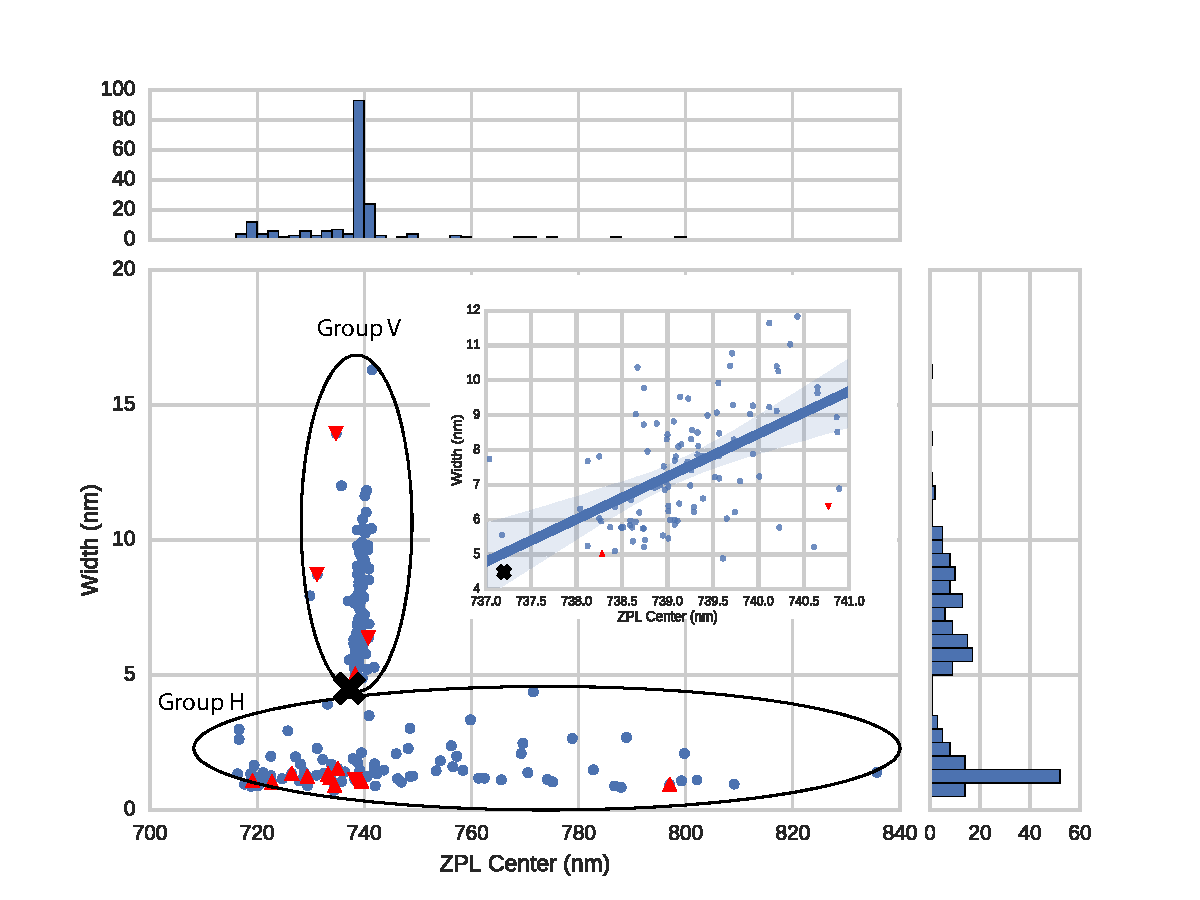
\includegraphics[trim = 0 0 0 0,  clip= true, width = 0.8\textwidth]{./pics/distro_histo_sarah_inset.pdf}}
		\caption{Distribution of the \lw vs. the center wavelength of the ZPL of the investigated \sivs in milled \nds containing \textit{in-situ} incorporated \sivs (samples \insituF, \insituS, \insituSn, \insituSo, \insituH{}). The data can be coarsely separated into two groups, H and V. The cross marks the position of an ideal \siv in unstrained bulk diamond \cite{Arend2016a}. The red triangles indicate emitters which exhibited an antibunching dip in the \gtz measurement. Upwards pointing triangles represent emitters which exhibit fluorescence intermittency (blinking), while triangles pointing down represent emitters which do not exhibit any blinking (see \autoref{subsec::photostab}). The inset displays a zoom into \vl, a least squares linear regression to the data, and the 95\% confidence interval of the regression as a shaded area around the fit line. A clear trend of broader \lws for longer \ZPL center shifts is visible.}
		\label{fig::bimodal_distr}
	\end{figure}


	\begin{figure}
		\begin{subfigure}[tp]{0.45\linewidth}
			\caption{}\label{subfig::emnarrow}
			\centering
			\testbox{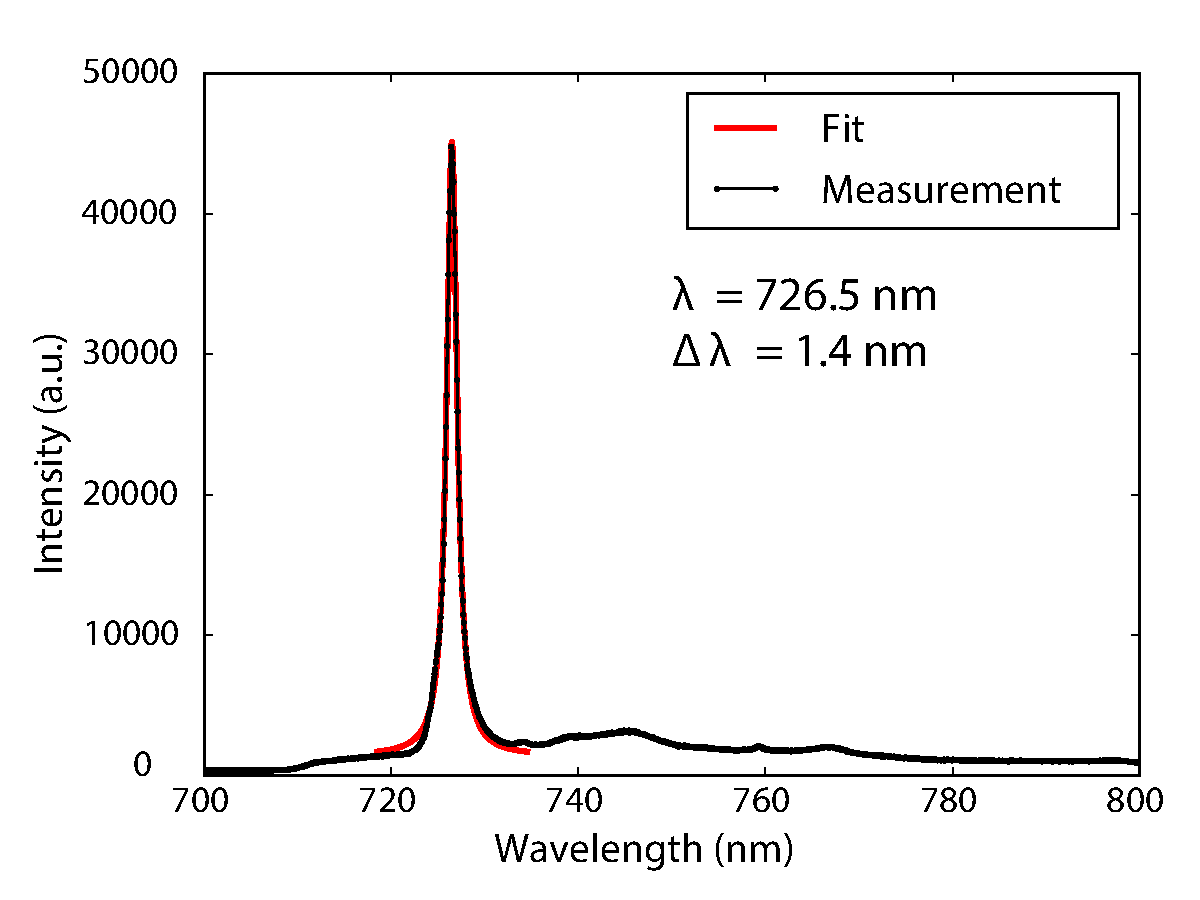
\includegraphics[trim = 0 0 0 0 , clip = true, width = \linewidth]{./pics/Ir8_Spektrum_8_notitle.pdf}}
		\end{subfigure}
		\hfill
		\begin{subfigure}[tp]{0.45\linewidth}
			\caption{}\label{subfig::embroad}
			\centering
			\testbox{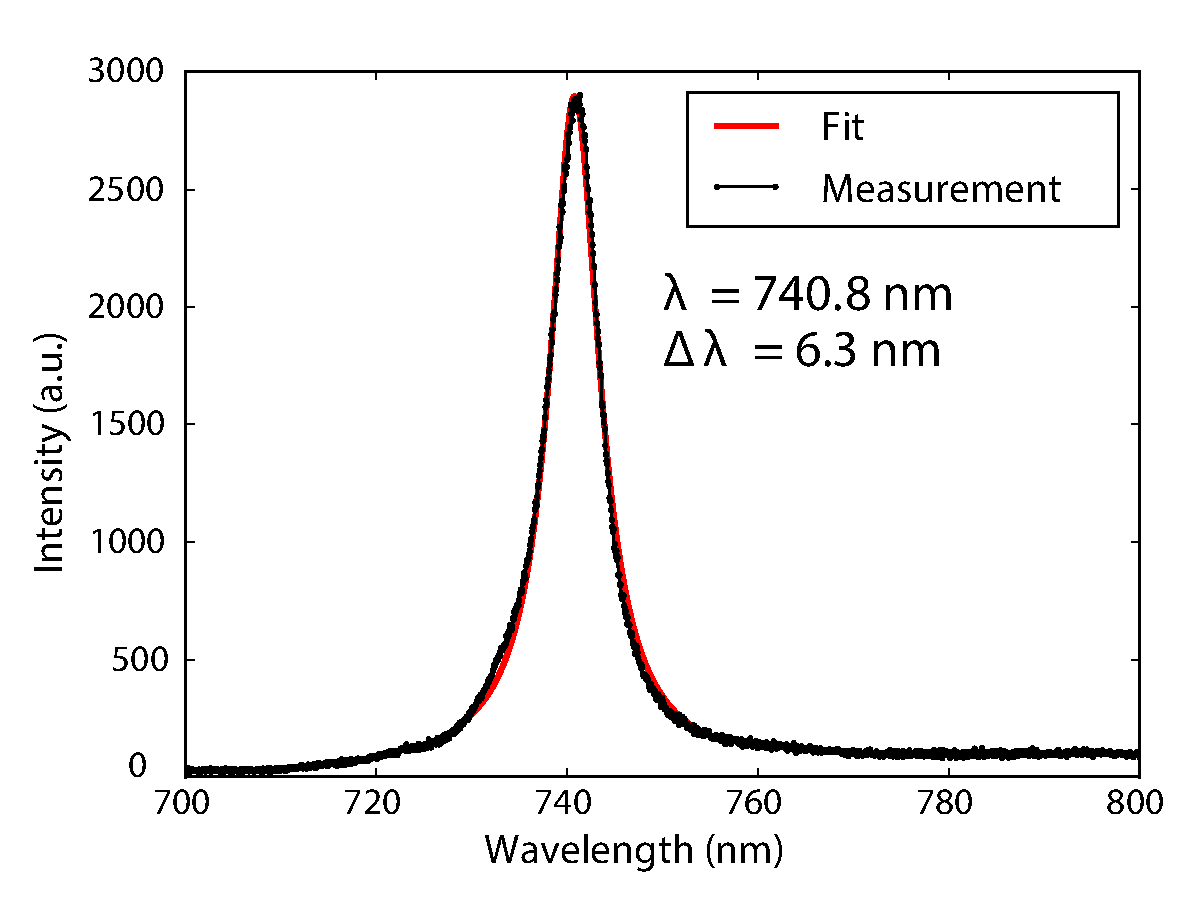
\includegraphics[trim = 0 0 0 0,  clip = true, width = \linewidth]{./pics/Ir8_scan_xy05_199uW_t30_notitle.pdf}}
		\end{subfigure}
		\caption{PL spectra measured with sample \insituHao. (a) A representative room temperature spectrum of one of the emitters in \hl of \autoref{fig::bimodal_distr}, denoted emitter \emnarrow. (b) A representative room temperature spectrum of one of the emitters in \vl of \autoref{fig::bimodal_distr}, denoted \embroad. The red lines are Lorentzian fits to the peaks.}
		\label{fig::spectra}
	\end{figure}

	\begin{figure}[tp]
		\centering
		\testbox{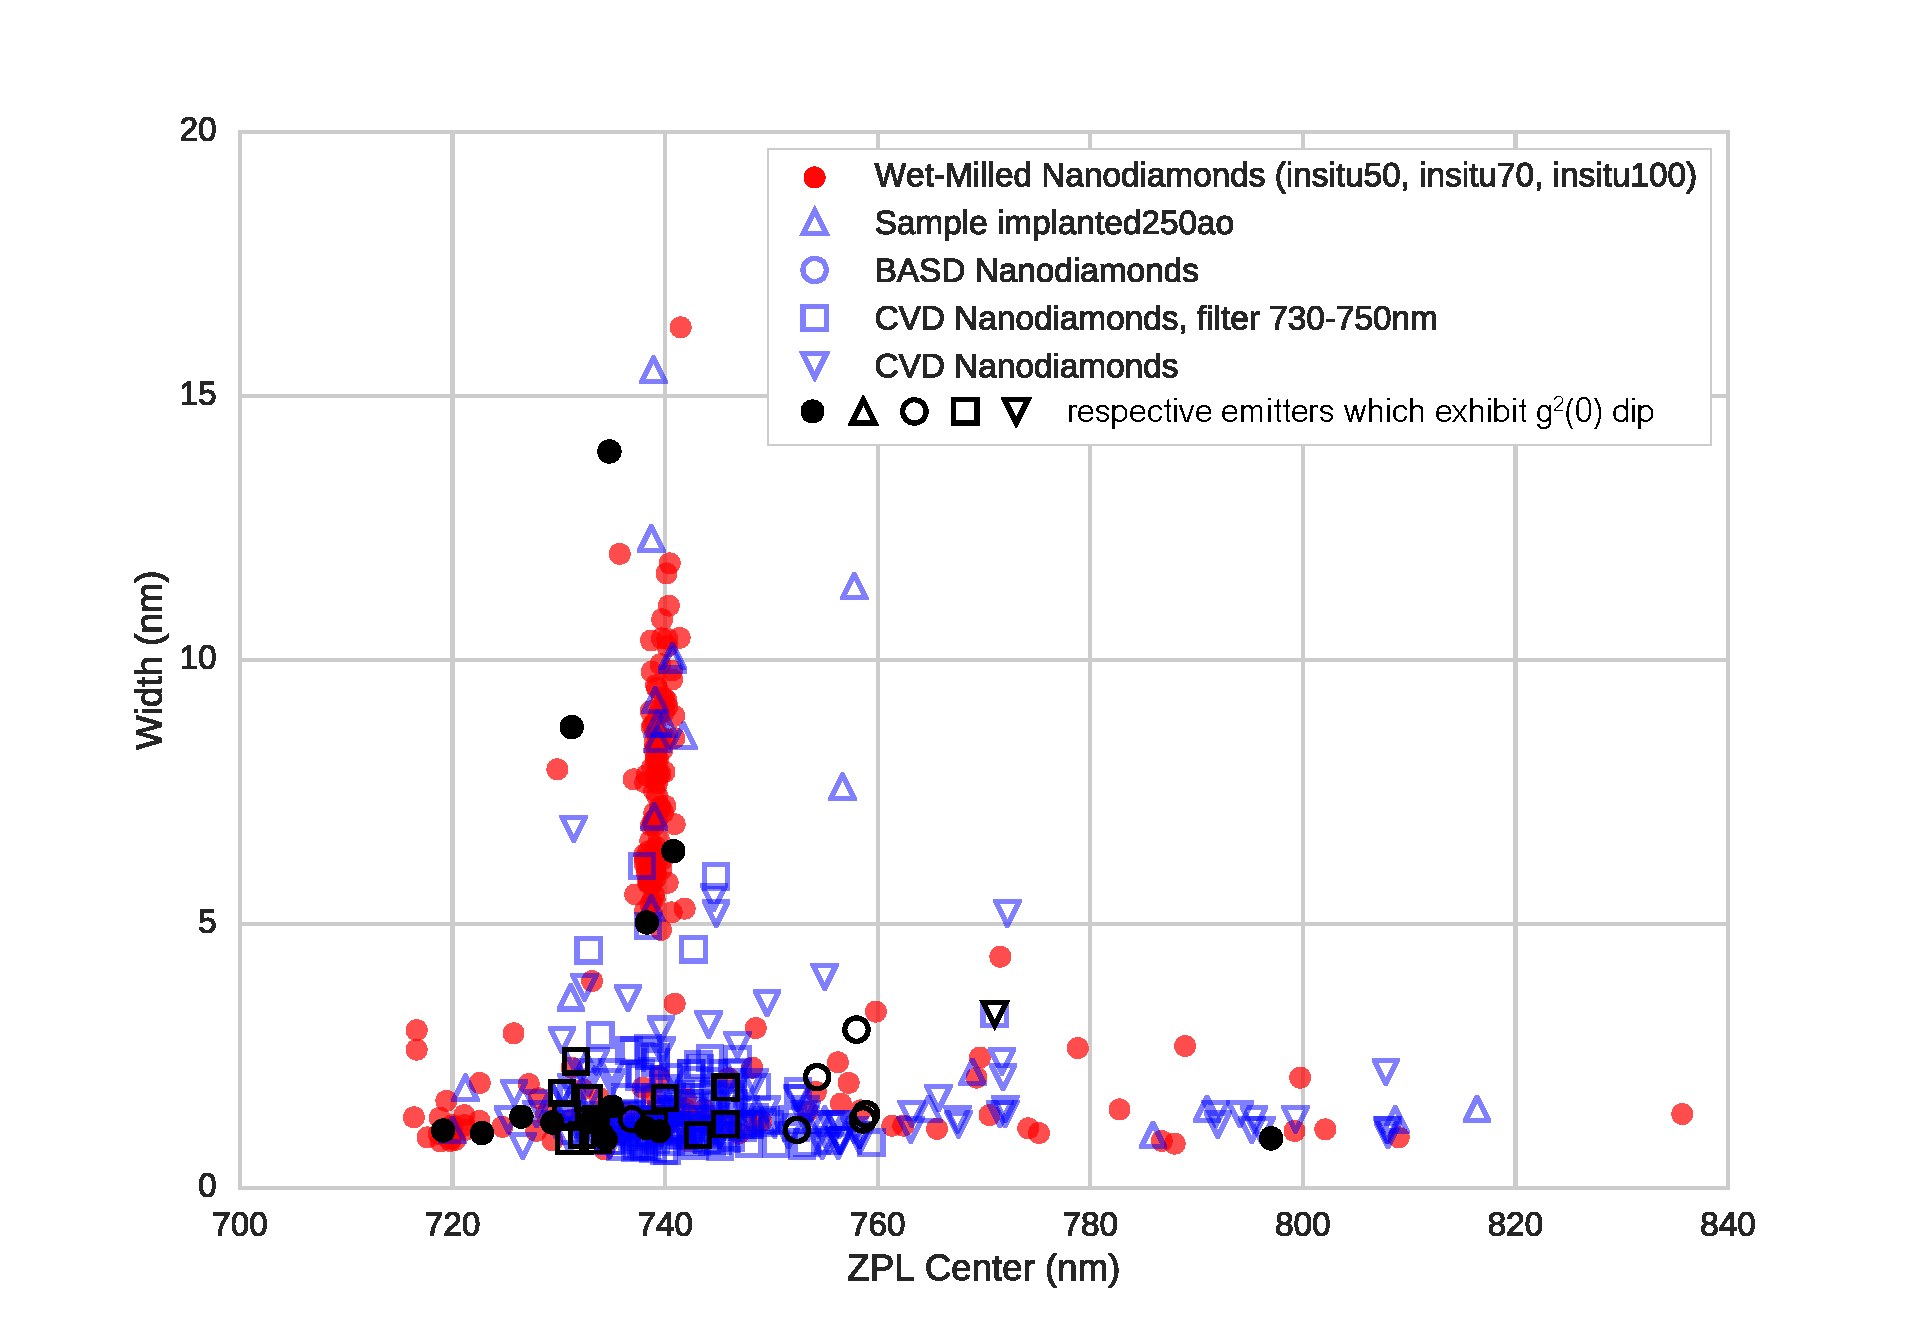
\includegraphics[trim = 0 0 0 0,  clip= true, width = 0.7\textwidth]{./pics/red_blue_markers_in_legend.pdf}}
		\caption{Comparison of the distribution of the \lw vs. the center wavelength of the ZPL of the investigated \sivs in milled \nds with data measured on the same \nds reported by J. Benedikter in \cite{Benedikter2017a}, with data measured on CVD \nds, with data measured in CVD diamonds by E. Neu in a filter window between \SIlist{730; 750}{nm} \cite{Neu2012}, and with data measured on \implantedTao, implanted with \Si. Black symbols represent emitters exhibiting a dip in the \gtz function, indicating a single or very few \sivs}
		\label{fig::bimodal_distr_compare}
	\end{figure}

	\begin{figure}[tp]
		\centering
		\testbox{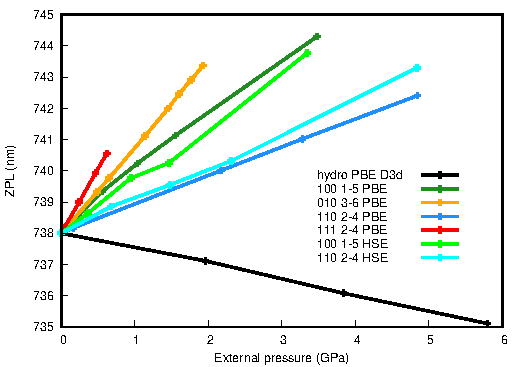
\includegraphics[trim = 0 0 0 0,  clip= true, width = 0.5\textwidth]{./pics/ZPL_shift_SiV_new.pdf}}
		\caption{Calculations of the wavelength of the \siv \ZPL in dependence of pressure. Black: hydrostatic pressure; other colors: uniaxial pressure, for different orientations and calculated with different functionals PBE and HSE. Hydrostatic-type pressure causes a moderate blue shift whereas uniaxial strain causes larger redshift with different magnitudes depending on the direction of the strain \correct{better description from Adam Gali}}
		\label{fig::stress_pressure}
	\end{figure}


	The \cwl and the \lw of the \zpl of each measured SiV luminescence spectrum of the samples \insituF, \insituS, and \insituH are determined by fitting a Lorentzian fit to the \ZPL.
	Both spectra from single and multiple \sivs are taken into account.
	The \lw of each ZPL is plotted against its \cwl (\autoref{fig::bimodal_distr}).
	What immediately strikes the eye is a pattern that to our knowledge has not been reported to date: 
	The observed ZPLs accumulate in two different regimes, namely a horizontal lobe (denoted \hl) and a vertical lobe (\vl) divided by a gap with hardly any data points. 
	Single emitters are found both in \hl and \vl (for more details about single emitters see section \ref{subsec::g2}).
	\\
	The two groups are defined by their characteristic \cwls and \lws: 
	In \hl very prominent ZPL peaks are found which show \lws between about \SIrange{1}{5}{nm} at \cwls which vary between about \SIrange{715}{835}{nm}.
	\autoref{subfig::emnarrow} shows a representative spectrum of a single emitter of \hl (denoted \emnarrow), exhibiting a ZPL line width of \SI{1.4}{nm} at a \cwl of \SI{726.5}{nm}.
	In contrast, in \vl, the spectra exhibit broader ZPL \lws of about \SI{5}{nm} up to \SI{18}{nm}.
	Their ZPL \cwls, however, are distributed within a very narrow range between \SIrange{738}{741}{nm}.
	\autoref{subfig::embroad} shows a spectrum of a single emitter of \vl (denoted \embroad), exhibiting a ZPL \lw of \SI{6.4}{nm} at a \cwl of \SI{740.8}{nm}.
	For comparison, the room temperature ZPL of \sivs in unstrained bulk diamond shows a \lw of \SIrange{4}{5}{nm} at a \cwl of \SI{737.2}{nm} marked with a cross in \autoref{fig::bimodal_distr} \cite{Arend2016a,Dietrich2014}. 
	\\
	We also investigated the \db of the reported spectra, which states the amount of emission light stemming from the \ZPL wrt. emission from sidebands.
	The \db of \emnarrow  amounts to \num[separate-uncertainty]{0.81(1)}, corresponding to a \hr factor of \num[separate-uncertainty]{0.21(1)} which is in good agreement with the values reported in \cite{Neu2011b}.
	The error is mainly due to background correction. 
	When zooming in to the spectrum of \embroad it shows, that it does not exhibit any sidebands, i.e. all emission goes into the ZPL. 
	Considering resolution limits of the spectrometer, the \db factor amounts to close to 100\%.
	It has to be pointed out, that we did not find any systematic difference of the \db factor between \hl and \vl.
	\\
	As the broad \ZPL distribution shown in \autoref{fig::bimodal_distr} is unreported so far, we compare the results both to previous measurements and a control sample fabricated by \si implantation.
	The comparison of current, earlier and control data is presented in \autoref{fig::bimodal_distr_compare}.
	Samples for which previous data has been taken are:
	\begin{enumerate}
		\item \nds produced by \basd (BASD) of polycrystalline \CVD diamond films (\cite{Neu2011a}; data taken from \cite{Benedikter2017a})
		\item \nds produced directly via a \CVD process with \textit{in-situ} incorporated \sivs; measured in a spectral filter window of \SIrange{730}{750}{nm} (data reused from \cite{Neu2012} with permission)
		\item \nds produced in the same manner as the sample above; spectroscopic measurement procedure the same as the one performed on the milled, \textit{in-situ} implanted samples (see \autoref{tab::samplenames}, \insituF etc.)
	\end{enumerate}
	All previous data from different \nd material fit nicely with the \ZPL distribution.
	To rule out that the two lobes in the distribution are no artifacts due to other elements incorporated into the \nds during the process, such as residue from other processes performed in the growth chamber or material abrasion from chamber parts and to verify that the observed luminescent defects are indeed \si related, we performed control experiments that were implanted with \si to form \sivs (sample \implantedTao).
	\autoref{fig::bimodal_distr_compare} shows that the implanted \sivs cover roughly the same spectral range as the grown-in centers, thereby providing strong evidence for the \si related origin of the defects.
	\\
	In the next paragraphs, the \ZPL distribution will be discussed in further detail.
	At first, the \ZPL \cwl shift is investigated.
	Very few of the measured data points in \vl sit at a shorter \cwl than the point attributed to an ideal \siv in unstrained bulk material.
	This means, a red-shift of the \ZPL of an \siv is more likely than a blueshift.
	Several mechanisms contribute to the \cwl shift, namely hydrostatic- and material strain.
	As explained in \autoref{subsec::raman}, we measured the Raman shift of samples \insituS and \implantedTao.
	These measurements indicate strain in the diamond lattice.
	\autoref{fig::stress_pressure} shows the calculated shift of the  \ZPL in dependence of pressure in the diamond lattice both for hydrostatic stress and for uniaxial stress.
	PBE and HSE are two different funtionals used for the calculations \todo{input Adam Gali}.
	From \autoref{fig::stress_pressure} it can be seen, the assumption stated in \autoref{subsec::raman} that the strain in the \nds is mainly due to uniaxial stress corresponds well with the measured \ZPL red-shift in \vl.
	With higher uniaxial pressure, the \ZPL becomes more and more red-shifted.
	However, the measured shifts in \hl are too broad to be solely explained by strain in the diamond.
	We suspect that there are other defect sites present in the vicinity of the \siv which explain the strong variation \cite{Thiering2015}.
	This statement is strengthened by the measurement of the shift of the first order Raman peak to lower wavenumbers.
	The investigation of this hypothesis presents an interesting topic for further research.
	\\
	Zooming in to \vl, another effect becomes visible (inset in \autoref{fig::bimodal_distr}):
	With increasing  \ZPL, the \lw becomes broader.
	The data points in \vl are fitted with a linear regression to guide to the eye.
	Linking the correspondence between the strain and the red-shift of the \ZPL with that of the slope of between the \cwl of the \ZPL and the \lw leads to the conclusion that also the \lw is affected by strain in the diamond lattice: The higher the uniaxial stress, the bigger the linewidth.
	\\
	To conclude, we are able to explain \vl very consistently with theoretical predictions for the \ZPL \cwl shift due to strain in the diamond lattice. 
	On the other hand, we suspect that \hl is due to lattice defects in the vicinity of the \siv, which has to be investigated in further research.
